Having established and validated the tools for the quantification of bovine \textit{IFITs} and elucidated the optimal assay termination time points for bRSV infections, we were equipped to replicate the analysis conducted in Chapter \ref{ch:Assessment of Transcriptional Induction of Human IFITs in the Context of RSV}. Our goal was to systematically assess the induction of \textit{bIFITs}, starting with different activators of the innate immune system, followed by bRSV infection, and finally, evaluating cross-species defence against hRSV infection. The relative induction levels were assessed using RT-qPCR methodology, as described in Section \ref{sec:Quantitative Real Time/Reverse Transcription PCR}. Briefly, cells were cultured in 12-well plates and exposed to the respective stimulants. At the endpoint of the experiments, RNA extraction was performed, followed by complementary DNA (cDNA) synthesis and transcript quantification through qPCR. The expression of \textit{hRSV N}, \textit{bRSV N}, and \textit{bMx1} genes was quantified using the $\Updelta$$\Updelta$Ct method, standardised to the bovine \textit{GAPDH} gene, and further normalised against mock-treated samples. As described previously, bovine \textit{IFIT} genes copy numbers were extrapolated from standard curves, created freshly per experiment, normalised relative to the mock copy numbers, and further standardised to the relative levels of bovine \textit{GAPDH} detected per experimental condition. The statistical analysis adhered to the procedures outlined in Section \ref{sec:Statistical Analysis}. It's important to note that the selection of the appropriate statistical test was contingent upon the assessment of data distribution normality and equality of variance, considerations that will be elaborated upon in the subsequent sections of this chapter.

\subsection{Bovine \textit{IFIT} Responses to Activators of Innate Immune Response} \label{subsec:Bovine IFIT Responses to Activators of Innate Immune Response}
The Madin-Darby bovine kidney (MDBK) cell line, derived from bovine renal epithelium in 1958 \cite{Madin1958EstablishedOrigin.}, serves as a well-established model system in bovine virology studies. We assessed the cells for the induction potential of bovine \textit{IFITs} along with bovine \textit{Mx1} using bovine IFN$\upalpha$ and LPS (bovine IFN$\upgamma$ was not commercially available). Bovine \textit{Mx1} was included in the analyses due to its status as an Interferon-Stimulated Gene (ISG), widely reported in immunology and virology studies, and as we observed minimal bovine \textit{IFIT} responses throughout the study, to ensure the cell lines had functioning internal pathways for ISG induction. Figure \ref{fig:MDBK responses to bIFNa} displays the \textit{bIFIT} and \textit{bMx1} responses to stimulation with bIFN$\upalpha$ at a concentration of 5 ng/mL (equivalent to 1,000 UI/mL of hIFN$\upalpha$) for either 3 or 6 hours.

The data reveals that all assayed genes were significantly upregulated biologically within 3 hours of induction, although the magnitude varied substantially. For the bovine \textit{IFITs}, all exhibited higher induction at 3 hours compared to 6 hours. The \textit{bIFITs} displayed a similar induction pattern to that observed in A549 cells, with \textit{bIFIT1} showing the strongest response, \textit{bIFIT2} and \textit{bIFIT3} displaying medium responses of similar amplitudes, and \textit{bIFIT5} exhibiting the lowest response. Notably, \textit{bIFIT1} showed the highest induction at 20-fold and 5-fold for 3 and 6 hours of incubation, respectively, and was the only bovine \textit{IFIT} that exhibited biologically significant induction at 6 hours. \textit{bIFIT2} and \textit{bIFIT3} were induced by 6-fold and 3.5-fold for 3 and 6-hour incubations with bIFN$\upalpha$ respectively, while \textit{bIFIT5} was induced by 4-fold and 2-fold for the same respective periods. Regarding \textit{bMx1}, its response surpassed that of the bovine \textit{IFITs}, showcasing a time-dependent induction increasing from 32-fold to 120-fold as the treatment continued. This shows that MDBK cells are capable of \textit{bIFIT} and \textit{bMx1} induction, albeit with differing temporal dynamics. However, these responses are modest, especially compared to the previously observed human \textit{IFIT} responses to IFN$\upalpha$.

\begin{figure}
    \centering
    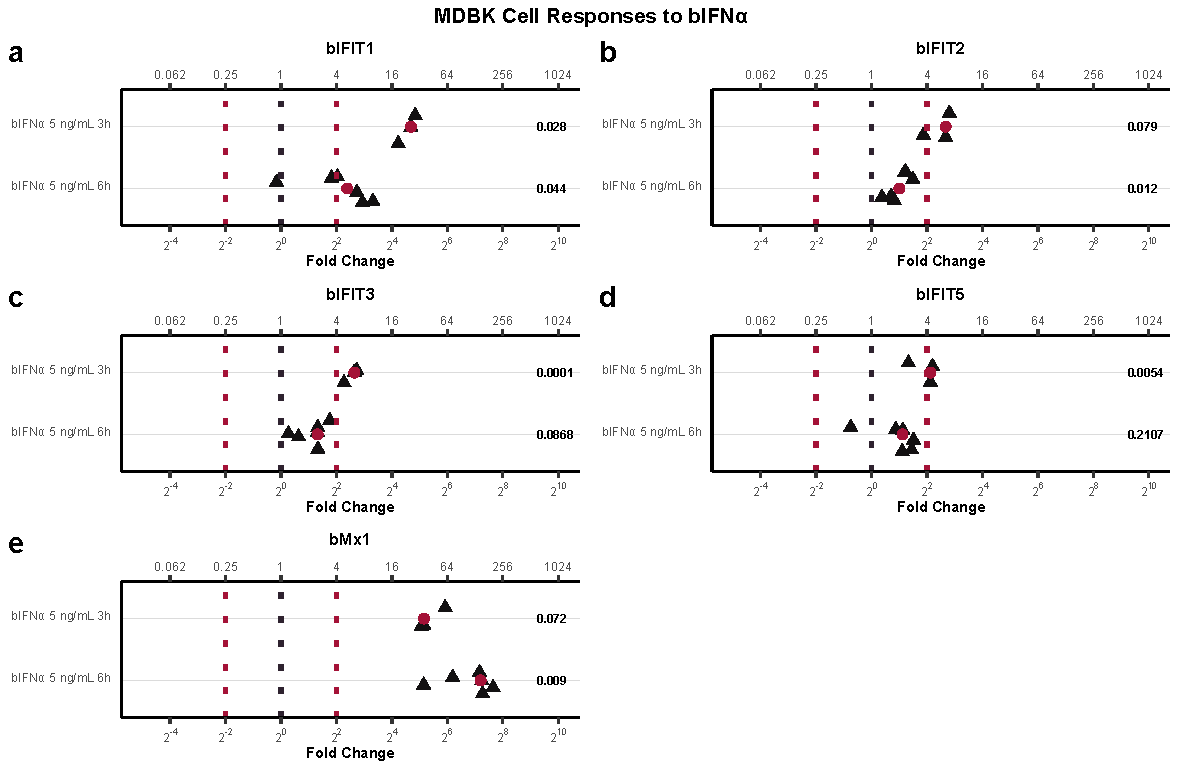
\includegraphics[width=1\linewidth]{07. Chapter 2/Figs/02. Induction/01. mdbk_treat_bifna.pdf}
    \caption[\textit{bIFIT} Gene Expression in MDBK Cells in Response to bIFN$\upalpha$ Stimulation.]{\textbf{\textit{bIFIT} Gene Expression in MDBK Cells in Response to bIFN$\upalpha$ Stimulation.} (a) \textit{bIFIT1}, (b) \textit{bIFIT2}, (c) \textit{bIFIT3}, (d) \textit{bIFIT5}, and (e) \textit{bMx1} gene expression levels were assessed using quantitative real-time PCR (qPCR) in MDBK cells following stimulation with bovine interferon alpha (IFN$\upalpha$) at a concentration of 5 ng/mL for a treatment duration of either 3 or 6 hours. Relative expression values are normalised to standardised mock-treated samples. Median values are represented by red circles. The black dotted line represents mock expression levels, while the red dotted lines indicate biologically significant induction thresholds. Numeric values indicate the p-values compared to mock-treated samples. While the datasets for \textit{bIFIT3} and \textit{bIFIT5} exhibited a normal distribution of data with equal variances, datasets for \textit{bIFIT1}, \textit{bIFIT2}, and \textit{bMx1} exhibited normal distributions with unequal variances.}
    \label{fig:MDBK responses to bIFNa}
\end{figure}

Furthermore, we aimed to investigate the involvement of Toll-like Receptor 4 (TLR4) in \textit{bIFIT} induction, previously observed to play a role in the A549 cell line (refer to Figure \ref{fig:A549 Response to LPS} in Section \ref{subsec:Human IFIT Responses to Activators of Innate Immune Response}). MDBK cells were incubated with LPS for 6 hours at concentrations of 0.5, 1, 2.5, 5, and 10 ng/mL. Subsequently, the cells were lysed, and their RNA was extracted, converted to cDNA, and quantified by qPCR as previously described. The obtained data is presented in Figure \ref{fig:MDBK responses to LPS}. Our findings indicate that neither \textit{bMx1} nor \textit{bIFITs} were induced to biologically significant levels by LPS within the tested concentration range. Most time points revealed no relative change, while 2.5 ng/mL resulted in a 50\% reduction in the levels of \textit{bIFIT1}, \textit{bIFIT2}, and \textit{bIFIT3}. Evidently, the data suggests that LPS, at the tested concentrations, does not induce \textit{bMx1} or \textit{bIFITs}; if anything, it causes a slight downregulation of their expression. 

\begin{figure}
    \centering
    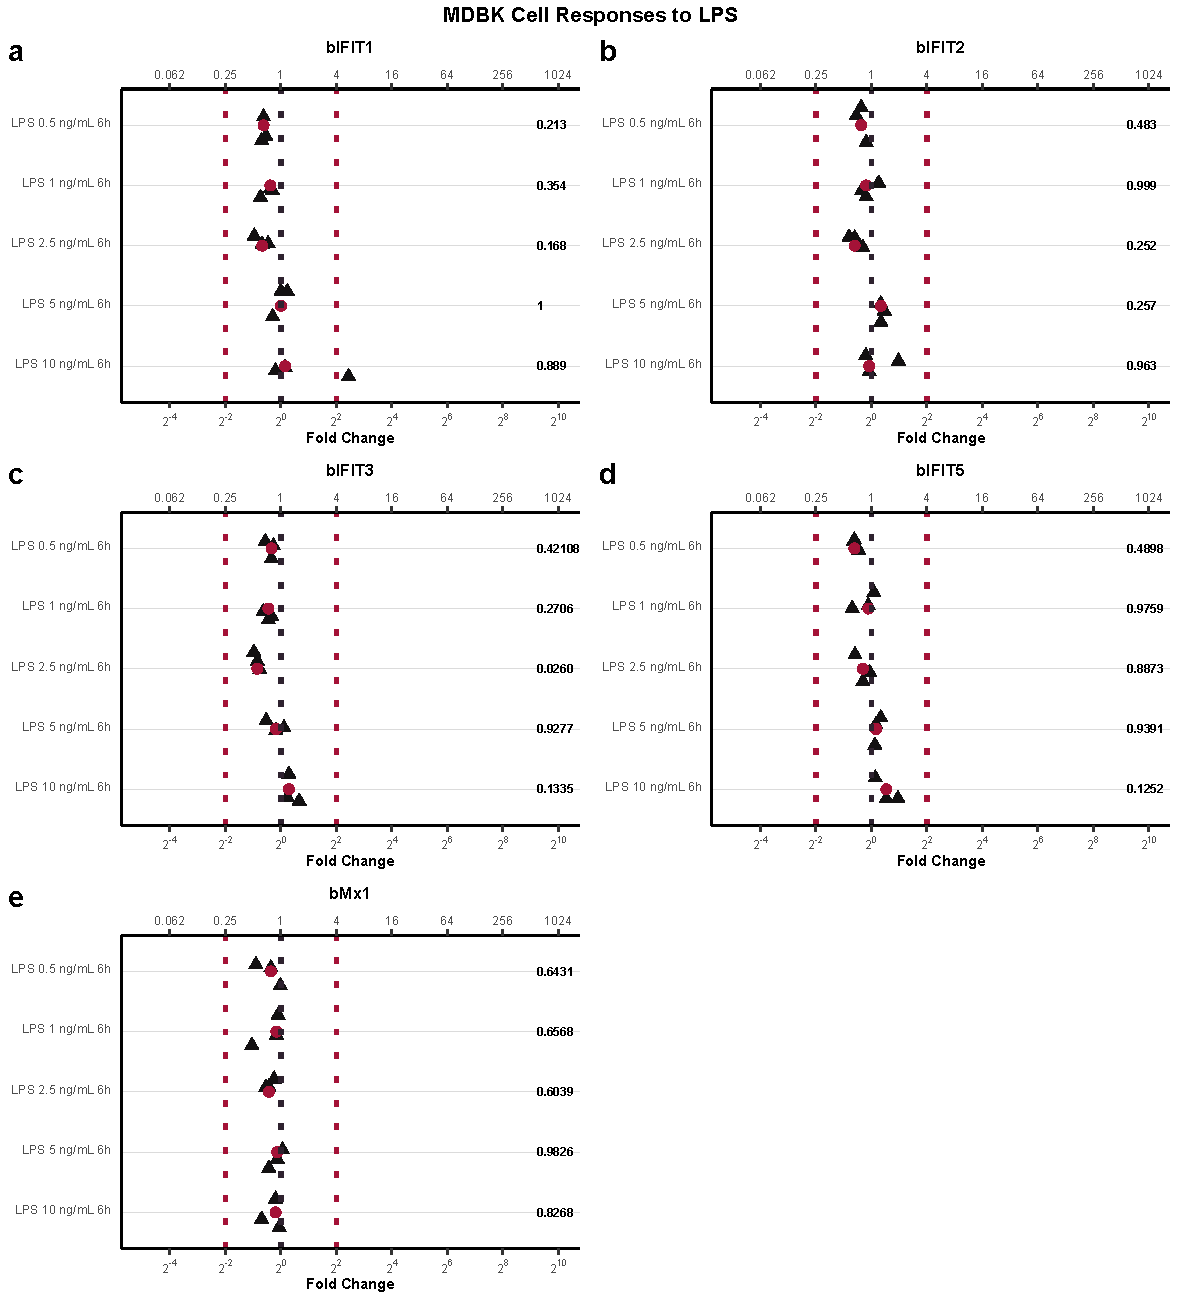
\includegraphics[width=1\linewidth]{07. Chapter 2/Figs/02. Induction/02. mdbk_treat_lps.pdf}
    \caption[\textit{bIFIT} Gene Expression in MDBK Cells in Response to LPS Stimulation.]{\textbf{\textit{bIFIT} Gene Expression in MDBK Cells in Response to LPS Stimulation.} (a) \textit{bIFIT1}, (b) \textit{bIFIT2}, (c) \textit{bIFIT3}, (d) \textit{bIFIT5}, and (e) \textit{bMx1} gene expression levels were assessed using quantitative real-time PCR (qPCR) in MDBK cells following stimulation with bacterial LPS at a concentration of 0.5, 1, 2.5, 5, and 10 ng/mL for a treatment duration of 6 hours. Relative expression values are normalised to standardised mock-treated samples. Median values are represented by red circles. The black dotted line represents mock expression levels, while the red dotted lines indicate biologically significant induction thresholds. Numeric values indicate the p-values compared to mock-treated samples. While the datasets for \textit{bIFIT3}, \textit{bIFIT5}, and \textit{bMx1} exhibited a normal distribution of data with equal variances, the datasets for \textit{bIFIT1} and \textit{bIFIT2} showed normal distributions with unequal variances.}
    \label{fig:MDBK responses to LPS}
\end{figure}

To validate the MDBK induction data, the BT cell line was employed. Originating from Bovine viral diarrhoea virus (BVDV) negative bovine nasal turbinate cells, isolated in 1974 from a neonatal Holstein cow \cite{McClurkin1974ComparisonVirus.}, these cells, mentioned in Section \ref{Growth Curves of Bovine RSV in Bovine Cell Lines}, facilitate bRSV replication and originate from a more physiologically significant site in the bRSV life cycle compared to the MDBK cell line. BT cells were incubated with 5 ng/mL of bIFN$\upalpha$ for either 3 hours or 24 hours. Figure \ref{fig:BT responses to bifna} depicts the results. At 3 hours of treatment, all genes, except \textit{bIFIT2}, were induced to biologically significant levels. However, after 24 hours, the relative mRNA levels returned to basal levels. Specifically, \textit{bIFIT1} displayed the highest response with a 20-fold induction, followed by \textit{bMx1} with a 16-fold increase. \textit{bIFIT3} showed an 8-fold induction, while \textit{bIFIT5} exhibited a 4-fold increase. In summary, it can be concluded that the BT cell line is sensitive to interferon and competent in \textit{bIFIT} induction. This data aligns with the MDBK data (Figure \ref{fig:MDBK responses to bIFNa}), revealing acute responses of \textit{bIFITs} to bIFN$\upalpha$ stimulation, although the induction is not sustained by 24 hours. Differences include the loss of induction persistence of \textit{bMx1}, the absence of bIFN$\upalpha$ sensitivity in \textit{bIFIT2}, and general lower responsiveness compared to the MDBK cell line.

\begin{figure}
    \centering
    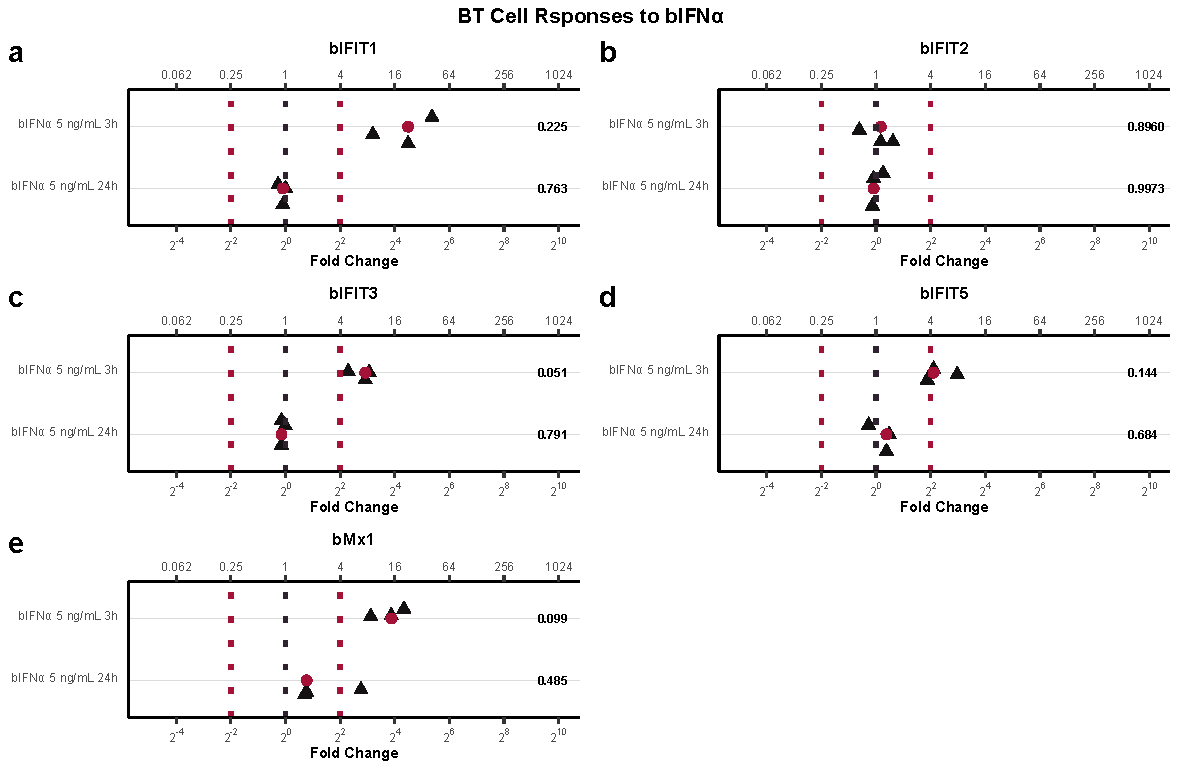
\includegraphics[width=1\linewidth]{07. Chapter 2/Figs/02. Induction/08. bt_bifna.pdf}
    \caption[\textit{bIFIT} Gene Expression in BT Cells in Response to bIFN$\upalpha$ Stimulation.]{\textbf{\textit{bIFIT} Gene Expression in BT Cells in Response to bIFN$\upalpha$ Stimulation.} (a) \textit{bIFIT1}, (b) \textit{bIFIT2}, (c) \textit{bIFIT3}, (d) \textit{bIFIT5}, and (e) \textit{bMx1} gene expression levels were assessed using quantitative real-time PCR (qPCR) in BT cells following stimulation with bovine interferon alpha (IFN$\upalpha$) at a concentration of 5 ng/mL for a treatment duration of either 3 or 24 hours. Relative expression values are normalised to standardised mock-treated samples. Median values are represented by red circles. The black dotted line represents mock expression levels, while the red dotted lines indicate biologically significant induction thresholds. Numeric values indicate the p-values compared to mock-treated samples. While the dataset for \textit{bIFIT2} displayed a normal distribution of data with equal variances, all other datasets showed normal distributions with unequal variances.}
    \label{fig:BT responses to bifna}
\end{figure}

\subsection{Bovine \textit{IFITs} Responses to Bovine RSV Infection} \label{subsec:Bovine IFITs Responses to Bovine RSV Infection}
Confirming the competence of the selected cell lines for \textit{bIFIT} induction, our goal was to evaluate the impact of bRSV infection on \textit{bIFIT} induction, particularly concerning varying viral MOIs and infection durations. To achieve this, MDBK cells were infected with crudely extracted bRSV at MOIs of 0.1, 1, and 2 for durations of 24 and 48 hours post-infection (HPI). The viruses employed in these experiments were prepared and quantified as detailed in Section \ref{subsec:Virus Propagation and Production} and Section \ref{subsec:Virus Quantification by TCID50 Assay}.

\begin{figure}
    \centering
    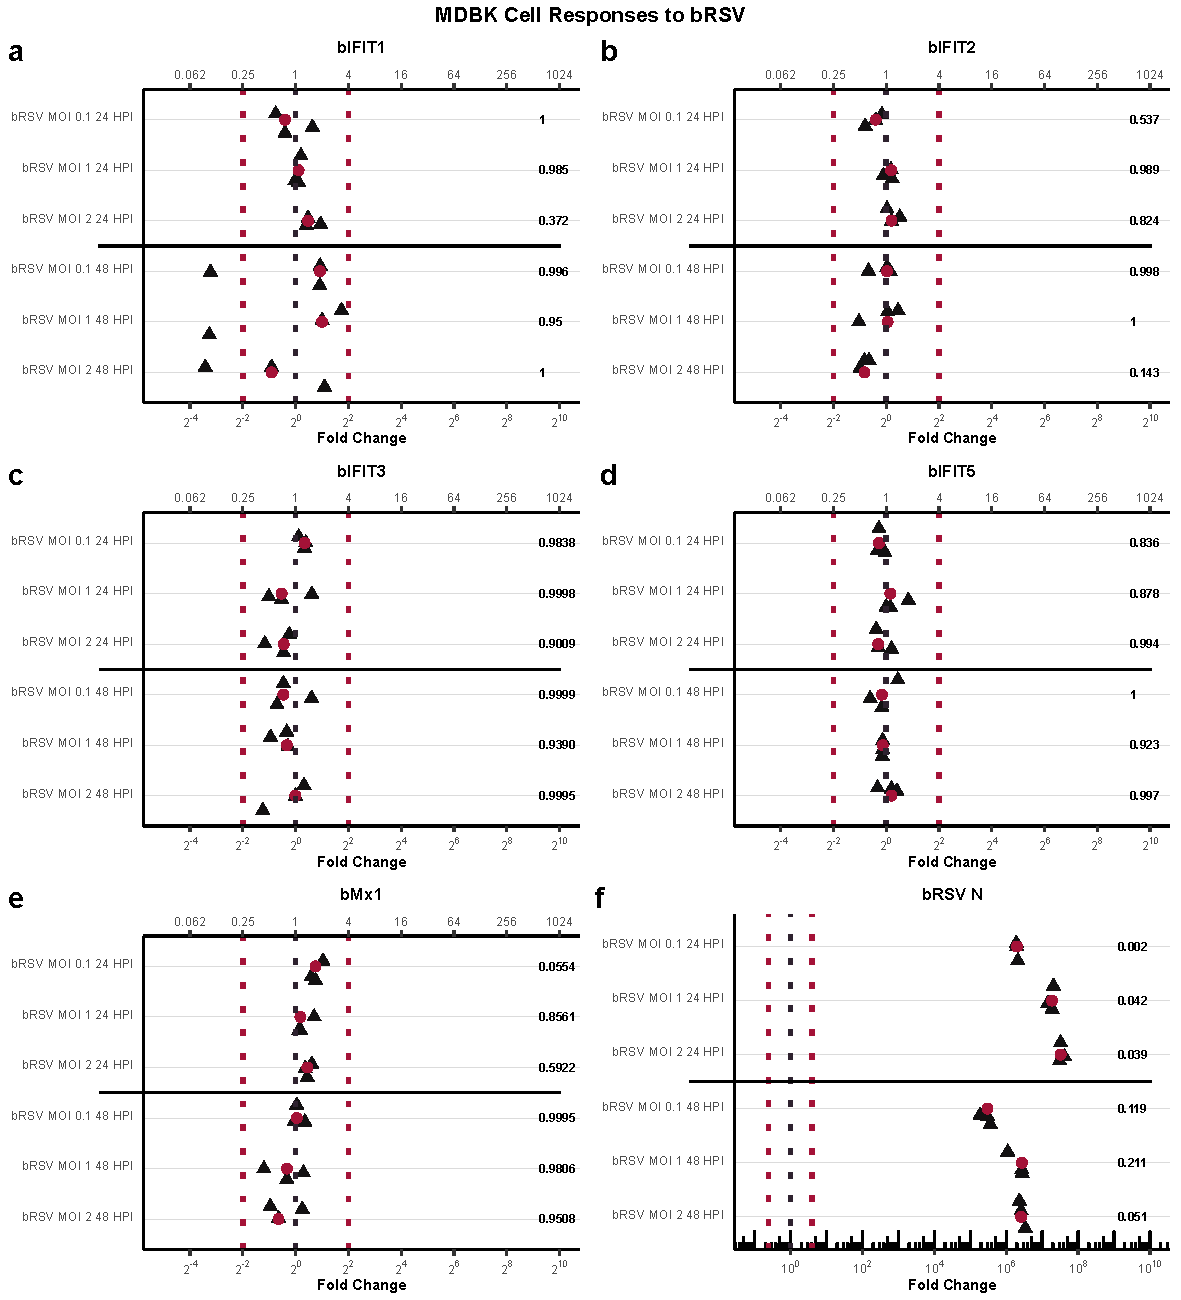
\includegraphics[width=1\linewidth]{07. Chapter 2/Figs/02. Induction/03. mdbk_brsv_timepoints.pdf}
    \caption[MDBK \textit{bIFIT} Response to bRSV Infection as a Function of Time and MOI.]{\textbf{MDBK \textit{bIFIT} Response to bRSV Infection as a Function of Time and MOI.} (a) \textit{bIFIT1}, (b) \textit{bIFIT2}, (c) \textit{bIFIT3}, (d) \textit{bIFIT5}, (e) \textit{bMx1} and (f) \textit{bRSV N} gene expression levels were assessed using quantitative real-time PCR (qPCR) in MDBK cell line following infection with bovine RSV at MOI of either 0.1, 1, or 2 for either 24 or 48 hours post-infection (delineated by the horizontal lines). Relative expression values are normalised to standardised mock-treated samples. Median values are represented by red circles. The black dotted line represents mock expression levels, while the red dotted lines indicate biologically significant induction thresholds. Numeric values indicate the p-values compared to mock-treated samples. From a statistical standpoint, the datasets for \textit{bIFIT3} and \textit{bMx1} showcased normal distributions and equal variances, while the others exhibited normal distributions with unequal variances.}
    \label{fig:MDBK responses to bRSV timepoints}
\end{figure}

The results of this experiment are depicted in Figure \ref{fig:MDBK responses to bRSV timepoints}. Evidently, while bRSV demonstrated successful replication, as indicated by the notably high relative \textit{bRSV N} values across all tested MOIs and timepoints (panel f), there were no biologically significant alterations in the mRNA levels of either \textit{bMx1} or \textit{bIFITs}. Specifically, while the mRNA levels of \textit{bIFIT3} and \textit{bIFIT5} remained unchanged under all conditions, minor positive and negative changes were observed in the expression of the other genes. Notably, \textit{bIFIT1} levels doubled for infections at 0.1 and 1 MOI at 48 HPI but decreased by half at MOI 2 at 48 HPI. \textit{bIFIT2} mRNA levels showed no significant changes except for the 2 MOI infection at 48 HPI. Additionally, \textit{bMx1} exhibited a two-fold induction in the case of 0.1 MOI infection at 24 HPI and a 50\% downregulation after 2 MOI infection at 48 HPI. The minimal responses to bRSV infection are intriguing, particularly considering our human data from Chapter \ref{ch:Assessment of Transcriptional Induction of Human IFITs in the Context of RSV}, which indicates that the \textit{hIFIT} responses are predominantly mediated by IFN$\upalpha$. Furthermore, as discussed in Section \ref{subsec:Bovine IFIT Responses to Activators of Innate Immune Response}, we are aware that \textit{bIFITs}, especially \textit{bMx1}, respond to bovine IFN$\upalpha$ stimulation. It is plausible that certain constituents within the bRSV or specific cytokines or chemokines in the crudely extracted bRSV preparations might impede the cascades necessary for \textit{bIFIT} induction.

\begin{figure}
    \centering
    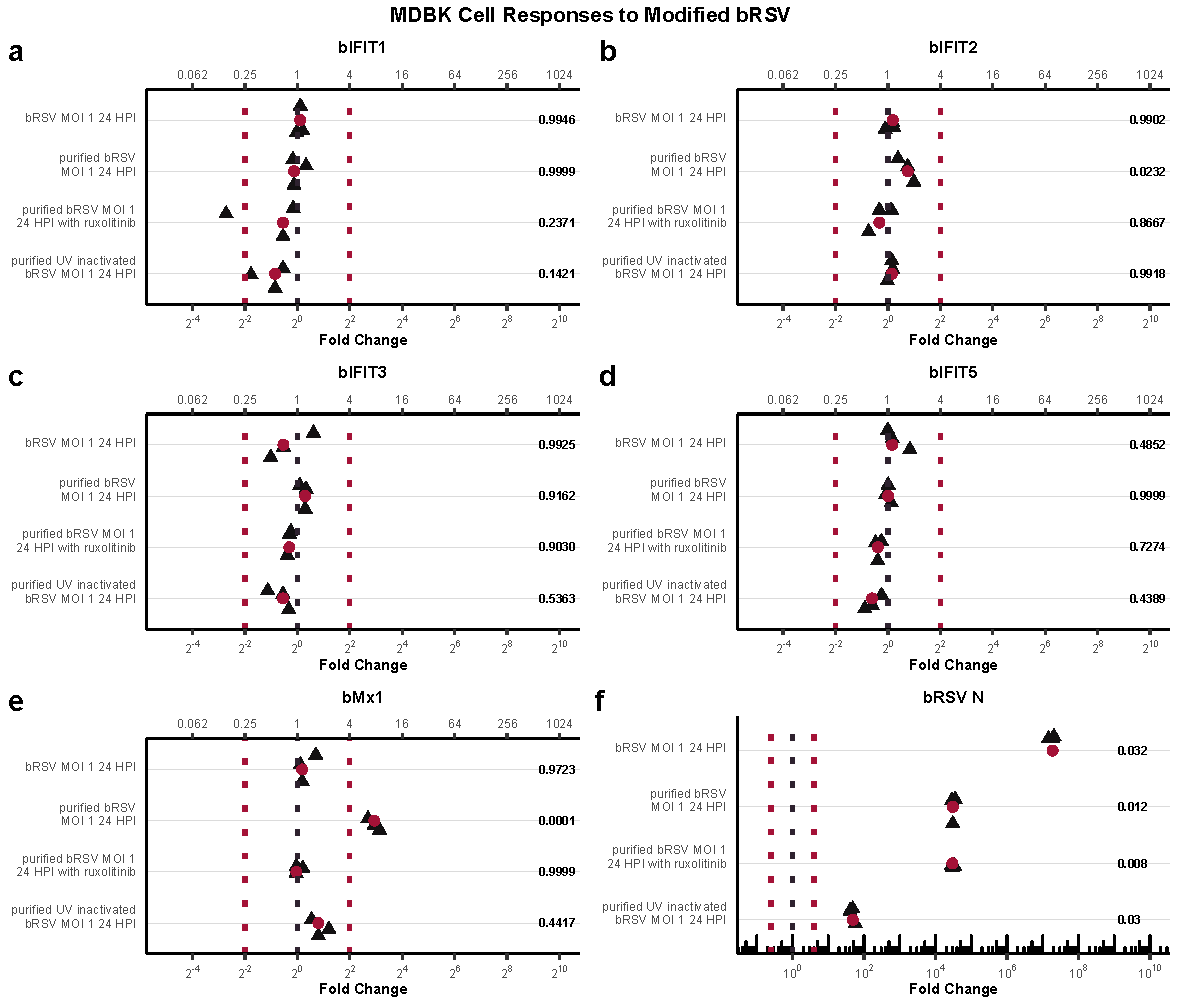
\includegraphics[width=1\linewidth]{07. Chapter 2/Figs/02. Induction/04. mdbk_brsv_uv_roxo.pdf}
    \caption[Impact of Ultra-Purification, UV-Inactivation, and INFR Inhibition on \textit{bIFIT} Induction in MDBK Cells Following bRSV Infection.]{\textbf{Impact of Ultra-Purification, UV-Inactivation, and INFR Inhibition on \textit{bIFIT} Induction in MDBK Cells Following bRSV Infection.} (a) \textit{bIFIT1}, (b) \textit{bIFIT2}, (c) \textit{bIFIT3}, (d) \textit{bIFIT5}, (e) \textit{bMx1}, and (f) \textit{bRSV N} gene expression levels were assessed using quantitative real-time PCR (qPCR) in MDBK cell line following infection with ultra-purified bRSV at MOI 1 for 24 hours. The cells were subjected to three different conditions: virus infection alone (top row), virus infection in the presence of 5 nM of ruxolitinib (interferon receptor inhibitor) throughout the infection (middle row), or UV-inactivated bRSV infection (bottom row). Relative expression values are normalised to standardised mock-treated samples. Median values are represented by red circles. The black dotted line represents mock expression levels, while the red dotted lines indicate biologically significant induction thresholds. Numeric values indicate the p-values compared to mock-treated samples. In terms of data distribution, while \textit{bRSV N} and \textit{bMx1} datasets exhibited normal distributions with unequal variances, the datasets for \textit{bIFIT1}, \textit{bIFIT2}, \textit{bIFIT3}, and \textit{bIFIT5} displayed normal distributions with equal variances.}
    \label{fig:The effect of ultra-purification, UV-inactivation and INFR inhibition on hIFIT induction following hRSV infection in MDBK}
\end{figure}

To investigate the possible influence of cellular contaminants on gene induction, MDBK cells were infected with ultrapurified bRSV, prepared through ultra-centrifugation on a discontinuous sucrose cushion as outlined in Section \ref{subsec:Virus Propagation and Production}. Simultaneously, we aimed to evaluate the impact of pharmacological inhibition of the interferon receptor and physical inactivation of bRSV on \textit{bIFIT} and \textit{bMx1} induction. This approach was prompted by our prior observation, as described in Section \ref{subsec:Human IFITs Responses to Human RSV} and illustrated in Figure \ref{fig:The effect of ultra-purification, UV-inactivation and INFR inhibition on hIFIT induction following hRSV infection in BEAS2B}, suggesting the requirement of basal interferon receptor activation for the maintenance of basal \textit{hIFIT} mRNA expression. The resultant data is displayed in Figure \ref{fig:The effect of ultra-purification, UV-inactivation and INFR inhibition on hIFIT induction following hRSV infection in MDBK}. Interestingly, the purification status of the virus did not influence the induction of \textit{bIFITs}. However, ultrapurification led to a seven-fold induction of \textit{bMx1}, a response that was entirely reversed by the presence of the interferon receptor inhibitor, ruxolitinib. Moreover, the presence of ruxolitinib marginally reduced the abundance of all \textit{bIFIT} mRNAs, though not to biologically significant levels. We observed a similar phenotype in the BEAS2B cell line (Section \ref{subsec:Human IFITs Responses to Human RSV}, Figure \ref{fig:The effect of ultra-purification, UV-inactivation and INFR inhibition on hIFIT induction following hRSV infection in BEAS2B}), where we concluded that the observed downregulation during ruxolitinib treatment was due to the higher basal \textit{IFIT} induction. Thus we can conclude the same with the MDBK cell line. Intriguingly, the relative median \textit{bRSV N} mRNA value remained consistent between the first two conditions, contrary to our observations in human samples where the presence of ruxolitinib amplified the relative median \textit{bRSV N} mRNA. Additionally, UV-inactivation of bRSV resulted in only minor changes for all genes, approximately around \(\pm\)2 in magnitude. Overall, the induction response of \textit{bMx1} mirrors what was observed with human RSV in A549 and BEAS2B cell lines in Chapter \ref{ch:Assessment of Transcriptional Induction of Human IFITs in the Context of RSV}. Conversely, we did not observe any significant alterations in the mRNA levels of \textit{bIFITs}. This suggests that certain cellular contaminants present in crudely extracted bRSV preparations were suppressing the induction of \textit{bMx1}, whereas their absence had no bearing on the potential inhibition of \textit{bIFIT} induction.

\begin{figure}
    \centering
    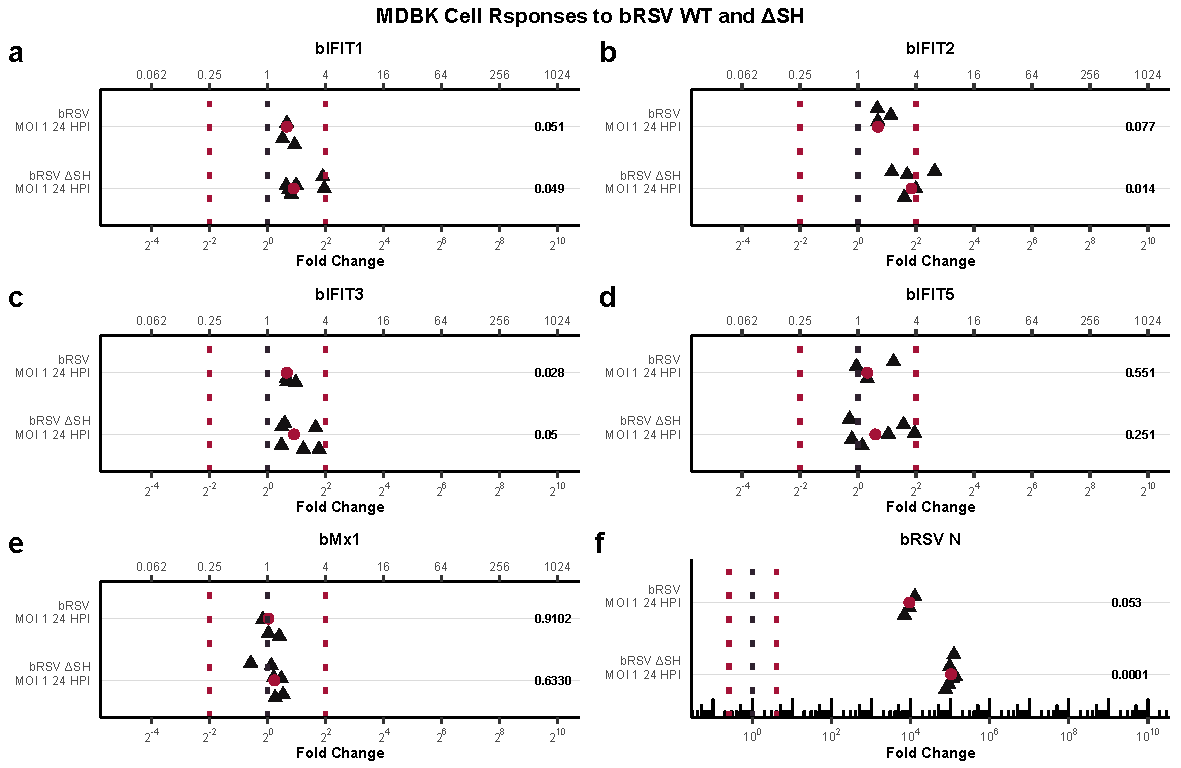
\includegraphics[width=1\linewidth]{07. Chapter 2/Figs/02. Induction/05. mdbk_brsv_moi1_dsh.pdf}
    \caption[MDBK \textit{bIFIT} Response to WT and $\Updelta$SH bRSV Infection.]{\textbf{MDBK \textit{bIFIT} Response to WT and $\Updelta$SH bRSV Infection.} (a) \textit{bIFIT1}, (b) \textit{bIFIT2}, (c) \textit{bIFIT3}, (d) \textit{bIFIT5}, (e) \textit{bMx1}, and (f) \textit{bRSV N} gene expression levels were assessed using quantitative real-time PCR (qPCR) in MDBK cell line following infection with WT or $\Updelta$SH bRSV at MOI 1 for 24 hours post-infection. Relative expression values are normalised to standardised mock-treated samples. Median values are represented by red circles. The black dotted line represents mock expression levels, while the red dotted lines indicate biologically significant induction thresholds. Numeric values indicate the p-values compared to mock-treated samples. Regarding data distribution, the \textit{bMx1} dataset exhibited a normal distribution of data with equal variances, while \textit{bIFIT1}, \textit{bIFIT2}, \textit{bIFIT3}, \textit{bIFIT5}, and \textit{bRSV N} datasets exhibited normal distributions with unequal variances.}
    \label{fig:MDBK responses to dSH}
\end{figure}

Next, our objective was to ascertain whether any of the bRSV genes inhibit the induction of \textit{bIFITs} or remain uninvolved during bRSV infection. As detailed in Section \ref{subsec:The Function of RSV Proteins}, key RSV proteins, namely SH, NS1, and NS2, play pivotal roles in modulating the host's innate immune response. For instance, the SH protein attenuates TNF-$\upalpha$ mediated signalling \cite{Fuentes2007FunctionProtein}, while NS1 and NS2 proteins interfere with the activation of the IFN gene promoter, inhibiting the phosphorylation of IRF3 \cite{Spann2005EffectsCytokines, Wright2006TheHumans}. NS1 operates in the nucleus, where it interacts with the gene regulatory domains of immune response genes, negatively influencing their transcription. Additionally, it disrupts the MAVS-RIG-1 complex on mitochondrial membranes and influences JAK/STAT signalling pathways through STAT2 degradation \cite{Pei2021Nuclear-localizedTranscription, Boyapalle2012RespiratoryInfection, Wright2006TheHumans}. NS2 plays a significant role in modulating cell morphology and increasing the dissemination of RSV virions \cite{Sedeyn2019RespiratoryResponses, Liesman2014RSV-encodedObstruction}. Recombinant RSV lacking NS1 and/or NS2 genes exhibits heightened sensitivity to interferon, increased apoptosis, and reduced replication efficiency \cite{Whitehead1999RecombinantChimpanzees, Teng2000RecombinantChimpanzees}. Our hypothesis posits that these proteins impede the induction of \textit{bIFITs}. To investigate this hypothesis, we utilised a panel of bRSV deletion mutants, including bRSV $\Updelta$SH, $\Updelta$NS1, $\Updelta$NS2, and the double deletion mutant $\Updelta$NS1/2, which were propagated and quantified as detailed in Section \ref{subsec:Virus Propagation and Production} and Section \ref{subsec:Virus Quantification by TCID50 Assay}. Due to the absence of non-structural proteins, lower final titers were obtained, necessitating infection at much lower MOIs. 

MDBK cells were infected with MOI 1 WT and $\Updelta$SH bRSV for 24 hours. Figure \ref{fig:MDBK responses to dSH} illustrates the relative mRNA changes of \textit{bIFITs} and \textit{bMx1} extracted from MDBK cells 24 HPI with MOI 1 WT and $\Updelta$SH bRSV. Both viruses demonstrated successful replication, with $\Updelta$SH bRSV exhibiting higher median relative mRNA levels at the experiment's endpoint compared to WT bRSV, contradicting the expected decreased fitness of this virus. However, \textit{bIFITs} and \textit{bMx1} responses to crudely extracted WT bRSV remained consistent with the previously observed minimal responses to the infection (see Figure \ref{fig:MDBK responses to bRSV timepoints}). Notably, $\Updelta$SH bRSV infection elicited no differential responses for any tested genes compared to WT bRSV infection, except for \textit{bIFIT2}, where median relative mRNA abundance increased to biologically significant levels at 4-fold.

\begin{figure}
    \centering
    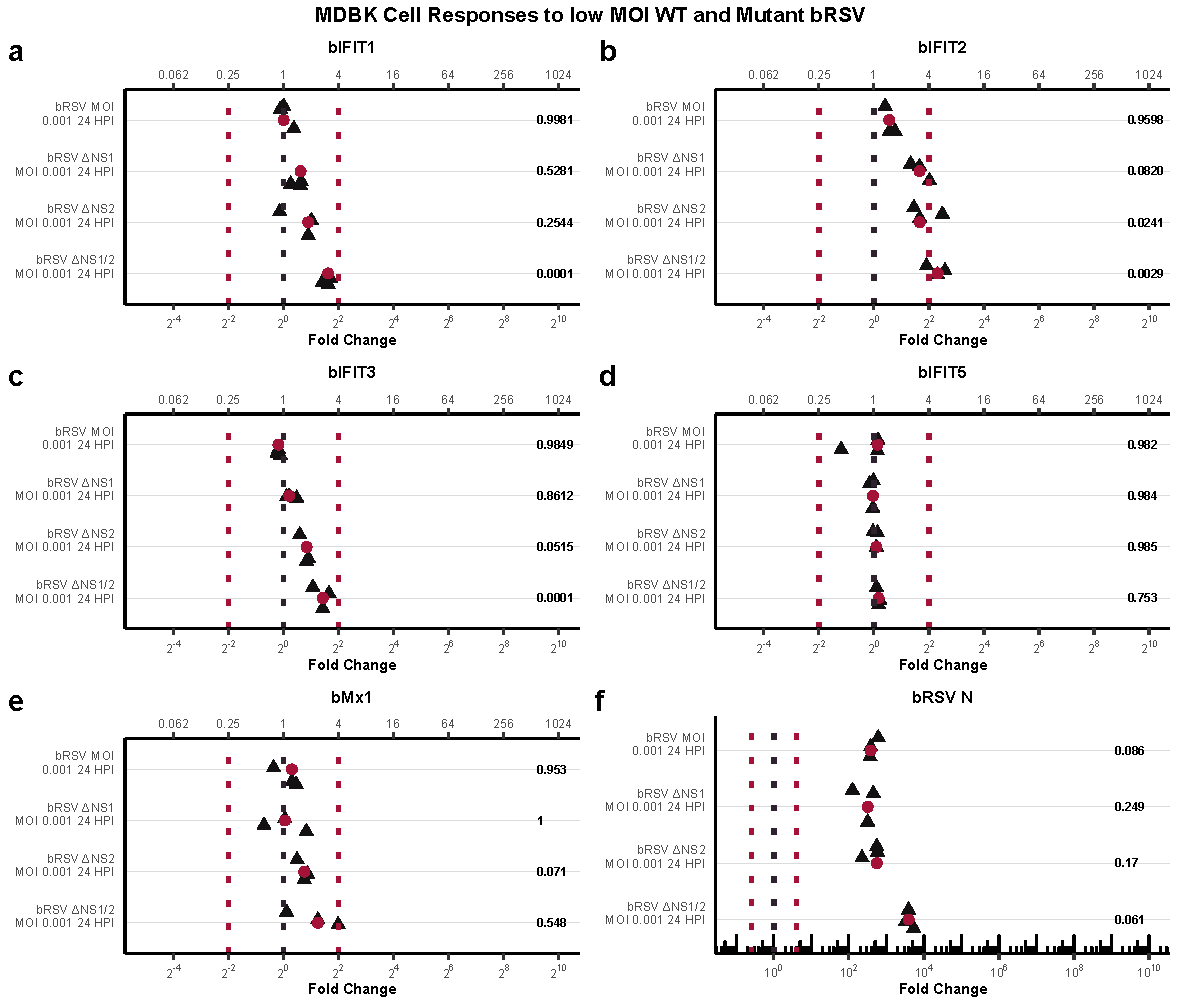
\includegraphics[width=1\linewidth]{07. Chapter 2/Figs/02. Induction/06. mdbk_brsv_low_moi.pdf}
    \caption[MDBK \textit{bIFIT} Response to Low MOI bRSV Infections.]{\textbf{MDBK \textit{bIFIT} Response to Low MOI bRSV Infections.} (a) \textit{bIFIT1}, (b) \textit{bIFIT2}, (c) \textit{bIFIT3}, (d) \textit{bIFIT5}, (e) \textit{bMx1}, and (f) \textit{bRSV N} gene expression levels were assessed using quantitative real-time PCR (qPCR) in MDBK cell line following infection with WT or $\Updelta$NS1, $\Updelta$NS2, and $\Updelta$NS1/2 bRSV at MOIs of 0.001 for 24 hours post-infection. Relative expression values are normalised to standardised mock-treated samples. Median values are represented by red circles. The black dotted line represents mock expression levels, while the red dotted lines indicate biologically significant induction thresholds. Numeric values indicate the p-values compared to mock-treated samples. Regarding data distribution, the \textit{bIFIT5}, \textit{bRSV N}, and \textit{bMx1} datasets exhibited a normal distribution of data with unequal variances, while the \textit{bIFIT1}, \textit{bIFIT2}, and \textit{bIFIT3} datasets exhibited normal distributions with equal variances.}
    \label{fig:MDBK responses to low MOI mutant bRSV}
\end{figure}

Continuing the investigation, we utilised 0.001 MOI $\Updelta$NS1, $\Updelta$NS2, and $\Updelta$NS1/2 bRSV along with 0.001 MOI WT bRSV as a control to assess their potential involvement in the suppression of \textit{bIFIT} induction. As illustrated in Figure \ref{fig:MDBK responses to low MOI mutant bRSV}, none of the genes of interest were influenced by WT infection, in line with our previous observations. Concerning the mutant viruses, \textit{bIFIT5} was unresponsive to any of them, while the other genes exhibited marginal induction in at least one condition. Notably, $\Updelta$NS1 infection influenced only \textit{bIFIT2}, inducing it nearly to biologically significant levels at around 3.8-fold. The absence of NS2 protein caused minor induction in all tested genes, except for \textit{bIFIT5}, approximately a 2-fold increase for \textit{bIFIT1}, \textit{bIFIT3}, and \textit{bMx1}, and a 3.8-fold induction for \textit{bIFIT2}. The infection with the double deletion mutant $\Updelta$NS1/2 bRSV resulted in the most robust response, inducing \textit{bIFIT1} and \textit{bIFIT3} at 3.8-fold, \textit{bMx1} at 3-fold, and notably, a biologically significant induction of \textit{bIFIT2} at 5-fold. This data suggests that, except for \textit{bIFIT5}, bRSV NS proteins negatively influence the induction of \textit{bIFITs} and \textit{bMx1}, with NS2 seemingly a more potent inhibitor.

\begin{figure}
    \centering
    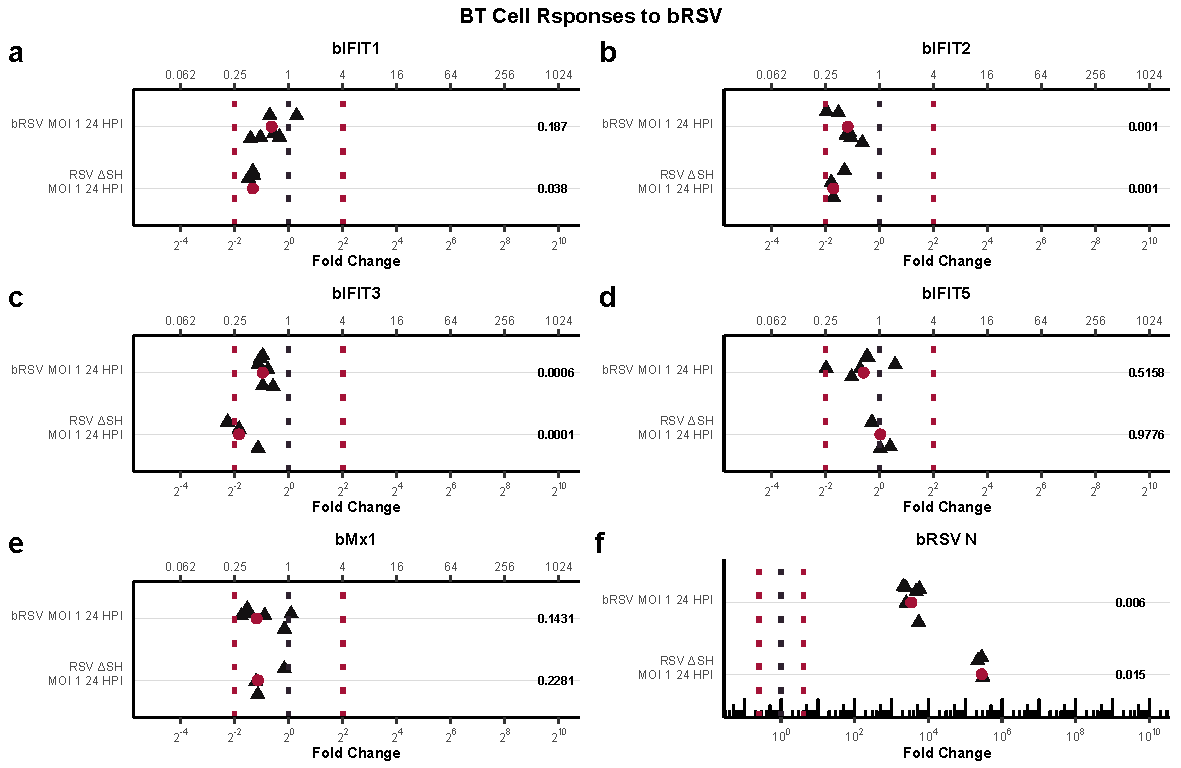
\includegraphics[width=1\linewidth]{07. Chapter 2/Figs/02. Induction/09. bt_brsv.pdf}
    \caption[BT \textit{bIFIT} Response to WT and $\Updelta$SH bRSV Infection.]{\textbf{BT \textit{bIFIT} Response to WT and $\Updelta$SH bRSV Infection.} (a) \textit{bIFIT1}, (b) \textit{bIFIT2}, (c) \textit{bIFIT3}, (d) \textit{bIFIT5}, (e) \textit{bMx1}, and (f) \textit{bRSV N} gene expression levels were assessed using quantitative real-time PCR (qPCR) in BT cell line following infection with WT or $\Updelta$SH bRSV at MOI 1 for 24 hours post-infection. Relative expression values are normalised to standardised mock-treated samples. Median values are represented by red circles. The black dotted line represents mock expression levels, while the red dotted lines indicate biologically significant induction thresholds. Numeric values indicate the p-values compared to mock-treated samples. All datasets exhibited normal distribution and equal variance except for \textit{bIFIT1} and \textit{bRSV N}.}
    \label{fig:BT responses to bRSV}
\end{figure}

Finally, we aimed to partially validate the bRSV infection data using the BT cell line. The cells were infected with crudely extracted WT and $\Updelta$SH bRSV at an MOI of 1 for 24 hours. The relevant data is depicted in Figure \ref{fig:BT responses to bRSV}.  In general, a reduction in mRNA levels was observed as a consequence of infection, regardless of the virus used. Specifically, WT bRSV infection led to a \(2^{-0.5}\)-fold decrease for \textit{bIFIT1} and \textit{bIFIT5}, a \(2^{-1}\)-fold decrease for \textit{bIFIT2} and \textit{bIFIT3}, and a \(2^{-1.5}\)-fold decrease for \textit{bMx1}. Infection with $\Updelta$SH bRSV resulted in approximately a \(2^{-1.5}\)-fold decrease in the levels of \textit{bIFIT1} and \textit{bMx1}, a biologically significant decrease of \(2^{-2}\)-fold for \textit{bIFIT2} and \textit{bIFIT3}, and no alteration in \textit{bIFIT5} mRNA levels. Overall, the presence of the SH protein appears to stimulate the induction of \textit{bIFIT} and \textit{bMx1}. This contrasts with observations in the MDBK cell line, where no differences were observed in the induction potential of WT and $\Updelta$SH bRSV, except for \textit{bIFIT2}, which was significantly upregulated in the absence of the SH protein (Figure \ref{fig:MDBK responses to dSH}).

\subsection{Bovine \textit{IFITs} Responses to hRSV Infection} \label{subsec:Bovine IFITs Responses to hRSV Infection}
We sought to investigate potential cross-species protection between hRSV and bRSV. As detailed in Section \ref{subsec:Human IFITs Responses to bRSV}, bRSV induces \textit{hIFITs} to a level surpassing that of equivalent hRSV infection in the A549 cell line, suggesting cross-protection of human cells to both viruses. While minimal \textit{bIFIT} or \textit{bMx1} responses were observed to WT or mutant bRSV infections in the MDBK and BT cell lines, we aimed to assess the potential response to hRSV. Furthermore, as noted in Section \ref{subsec:Human IFITs Responses to Human RSV}, the purification methodology for isolating hRSV influenced \textit{hIFIT} induction, with ultrapurified preparations causing higher levels of induction. Considering these factors, MDBK and BT cells were infected with crude extracted and ultracentrifugation-purified hRSV at an MOI of 1 for 24 hours. Subsequently, cells were lysed, mRNA was extracted and converted into cDNA, and transcripts were quantified using RT-qPCR.

\begin{figure}
    \centering
    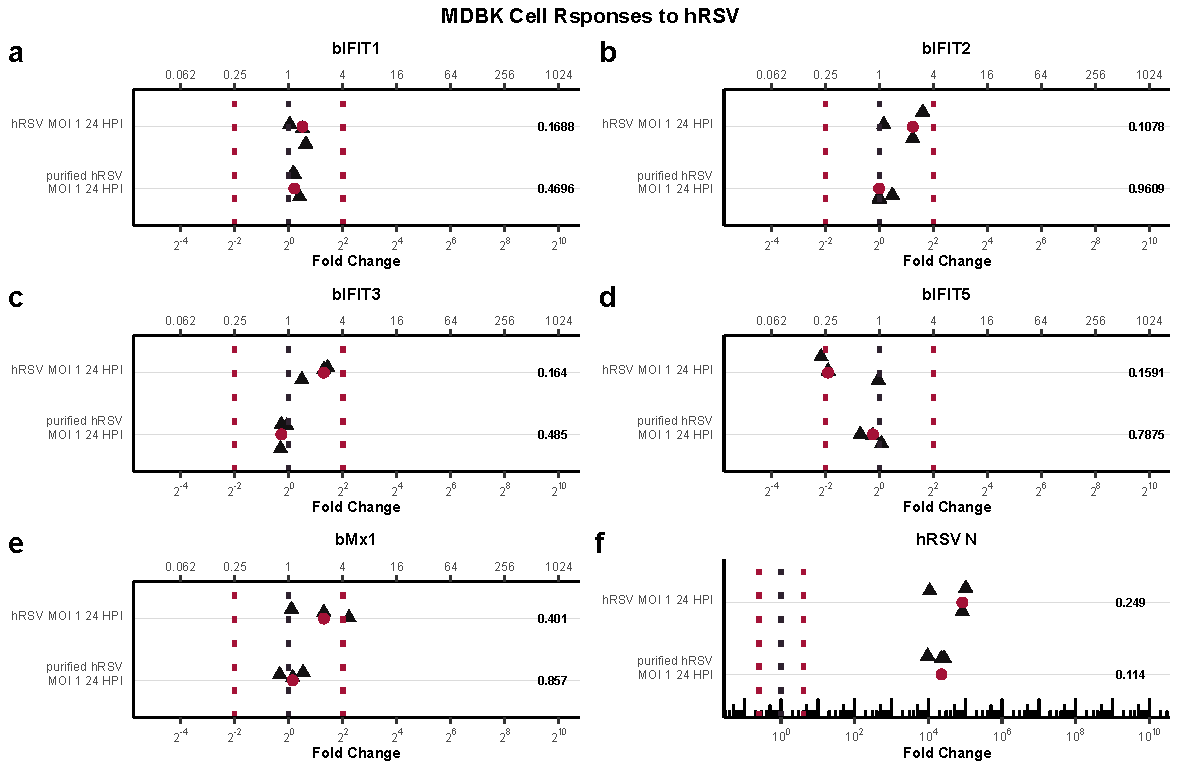
\includegraphics[width=1\linewidth]{07. Chapter 2/Figs/02. Induction/07. mdbk_hrsv.pdf}
    \caption[MDBK \textit{bIFIT} Response to Crude-Extracted and Ultra-Purified hRSV Infection.]{\textbf{MDBK \textit{bIFIT} Response to Crude-Extracted and Ultra-Purified hRSV Infection.} (a) \textit{bIFIT1}, (b) \textit{bIFIT2}, (c) \textit{bIFIT3}, (d) \textit{bIFIT5}, (e) \textit{bMx1}, and (f) \textit{hRSV N} gene expression levels were assessed using quantitative real-time PCR (qPCR) in MDBK cell line following infection with crude-extracted and ultra-purified hRSV at MOI 1 for 24 hours post-infection. Relative expression values are normalised to standardised mock-treated samples. Median values are represented by red circles. The black dotted line represents mock expression levels, while the red dotted lines indicate biologically significant induction thresholds. Numeric values indicate the p-values compared to mock-treated samples. The datasets for \textit{bIFIT1}, \textit{bIFIT2}, and \textit{bIFIT3} exhibited normal distributions with equal variances, while the rest displayed normal distributions with unequal variances.}
    \label{fig:bIFIT responses to hRSV infection in MDBK}
\end{figure}

Figure \ref{fig:bIFIT responses to hRSV infection in MDBK} illustrates the responses of \textit{bIFITs} and \textit{bMx1} to hRSV in MDBK cells. Both viral preparations successfully replicated, as evidenced by the quantification of \textit{hRSV N} (Panel f; \(2^{5}\)-fold and \(2^{4.2}\)-fold increases, respectively), albeit unexpectedly exhibiting an order of magnitude difference in the final fold changes. Notably, ultrapurified hRSV infection did not influence the relative levels of any tested genes. In contrast, crude extracted hRSV infection induced a variety of effects: a modest induction of \textit{bIFIT1} by 1.5-fold, and \textit{bIFIT2}, \textit{bIFIT3}, and \textit{bMx1} by 3-fold, alongside a significant downregulation of \textit{bIFIT5} by \(2^{-2}\)-fold.

\begin{figure}
    \centering
    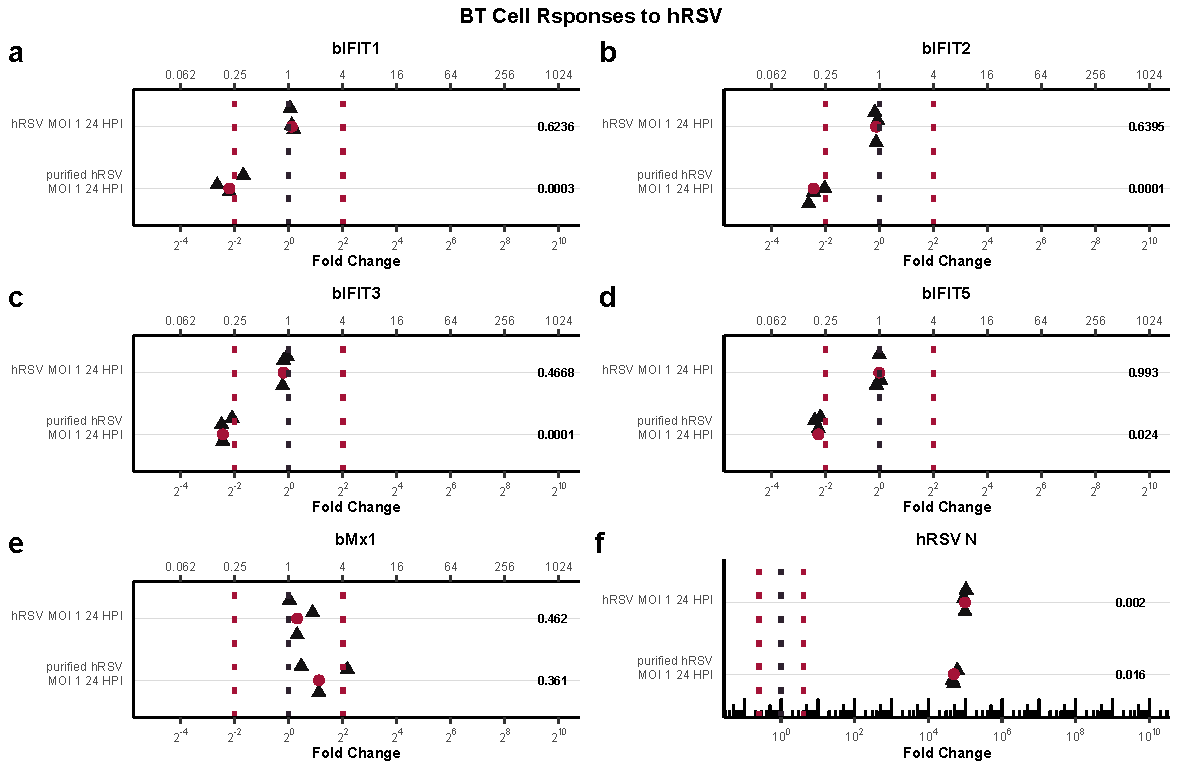
\includegraphics[width=1\linewidth]{07. Chapter 2/Figs/02. Induction/10. bt_hrsv.pdf}
    \caption[BT \textit{bIFIT} Response to Crude-Extracted and Ultra-Purified hRSV Infection.]{\textbf{BT \textit{bIFIT} Response to Crude-Extracted and Ultra-Purified hRSV Infection.} (a) \textit{bIFIT1}, (b) \textit{bIFIT2}, (c) \textit{bIFIT3}, (d) \textit{bIFIT5}, (e) \textit{bMx1}, and (f) \textit{hRSV N} gene expression levels were assessed using quantitative real-time PCR (qPCR) in BT cell line following infection with crude-extraccted and ultra-purified hRSV at MOI 1 for 24 hours post-infection. Relative expression values are normalised to standardised mock-treated samples. Median values are represented by red circles. The black dotted line represents mock expression levels, while the red dotted lines indicate biologically significant induction thresholds. Numeric values indicate the p-values compared to mock-treated samples. Normal distribution with equal variances was observed for \textit{bIFIT1} and \textit{bIFIT2} datasets, while the others exhibited normal distributions with unequal variances.}
    \label{fig:Bt responses to hRSV}
\end{figure}

Results from BT cells infected with hRSV are depicted in Figure \ref{fig:Bt responses to hRSV}. Similar to MDBK cells, hRSV successfully infected and replicated in BT cells. Interestingly, the effect observed in MDBK cells (Figure \ref{fig:bIFIT responses to hRSV infection in MDBK}) was reversed: the crude extracted viral preparation did not influence the expression of the genes of interest, while ultra-purified hRSV caused significant effects. It led to a biologically substantial downregulation of \textit{bIFIT1}, \textit{bIFIT2}, \textit{bIFIT3}, and \textit{bIFIT5} by \(2^{-2.5}\)-fold, and induced \textit{bMx1} by 2-fold.